\section{Related work on unsupervised approaches} \label{subject_indexing}

\acrfull{si} has been a topic in academia well before it became important in the digital realm, as it was relevant for the organization of conventional libraries. The current ISO standard (ISO 5963:1985) defines \acrshort{si} as a three-step process:

\begin{enumerate}
    \item Determine the content of a document.
    \item Perform conceptual analysis to extract concepts from the content.
    \item Translate the concepts into a controlled vocabulary.
\end{enumerate}

Automatic Subject Indexing (ASI) occurs when machines perform this \acrshort{si} procedure instead of humans. There are also approaches in which machines aid humans in the process of indexing, called Machine-Aided Indexing (MAI) or Computer-Aided Indexing (CAI). We will however refer to the automatic task as \acrshort{si}, which is how it is usually referred to in the literature. Indexing can be differentiated from classification in its purpose \cite{golub2019automatic}. It focuses on facilitating the retrieval of a document, assuming that users will look for it from different perspectives. Classification, on the other hand, tries to clearly categorize the documents, using fewer subjects per document and aiming for the highest precision instead of covering a broader spectrum of possible queries.

In this chapter, we review the literature on this topic. We first summarize the different ways in which \acrshort{si} methods can be classified, which revolve around two conditions: the existence of training data, which enables the implementation of supervised \acrlong{ml} algorithms, and the availability of a set of subjects. If such a set does not exist, the subjects must be extracted from the texts.

Afterwards, we present the common challenges that \acrshort{si} methods face. Heterogeneous documents increase the complexity of performing \acrshort{si}, whereas the number of documents hinders the performance of many methods. Also, texts written in different styles pose different problems. Subjects can also pose challenges, such as their uneven assignment distribution and how their distribution changes over time. Training data may also suffer from this distribution drift over time, as well as label noise due to inconsistencies between different human indexers.

In the next section, we present several unsupervised approaches to \acrshort{si} that use an existing set of subjects. We first present two approaches that are popular in the literature: string matching methods that map subjects to documents, relying on the quality of the set of subjects to achieve a high matching rate, and the application of \acrlong{lda} for subject indexing scenarios where subjects already exist.

We then present the \acrfull{mag} in section \ref{subject_indexing_mag}. The \acrshort{mag} is, to the best of our knowledge, the most successful application of unsupervised subject indexing for scientific texts. Its use case closely resembles ours, as their dataset comprises documents from various scientific fields. They are also the source for our set of subjects. Their indexing procedure consists of vectorizing documents and subjects and computing the cosine distances between them to discover the similarity between each document and each subject. In this thesis, we implement the \acrshort{mag} indexing procedure, as its scenario closely resembles ours, and it is proven to be accurate. The other approaches discussed in this chapter neither as accurate, nor as well tested for scientific texts. The \acrshort{mag} is widely used in academia to this day, so we safely assume its indexing method was successful.

\subsection{Classifications of methods} \label{subject_indexing_types}

% Subject indexing methods can be classified in various manners. For instance, approaches can be classified regarding the origin of the used subjects \cite{golub2019automatic}. Derived \acrshort{si} extracts the subjects from the document itself, while assigned \acrshort{si} maps a fixed set of subjects to the given document.

In this section, we give an overview of the different classifications of \acrshort{si} methods that we have found in the literature. They all revolve around the existence of a \acrfull{kos}, and the availability of training data.

\subsubsection{Golub's classification} \label{subject_indexing_golub}

Golub classifies \acrshort{si} approaches regarding the application purpose, the amount of research backing it and the paradigm used (\acrlong{ml} or string matching, essentially) \cite{golub2019automatic}. It classifies \acrshort{si} approaches into three groups.

\textit{Document clustering} is suited for cases where there is neither training data nor a \acrshort{kos}. Clustering algorithms group documents according to a given similarity metric. They can be used to group documents that belong to the same topic. For example, the similarity metric may measure the amount of mutual information between documents \cite{slonim2002unsupervised}. Document clustering poses two challenges: the resulting structures may be hard to understand \cite{chen2000bringing}, and they can also change once more documents are added. The second challenge is that the assignment of topics to clusters may be unclear and require human intervention.

\textit{Text categorization} is used when both training data and a \acrfull{kos} are available. It consists of a supervised \acrshort{ml} algorithm that learns the features of the subjects of the \acrshort{kos} from the already assigned documents. Once the algorithm is trained, these features will enable it to map subjects to new documents. It can be applied for \acrshort{kos}s that order subjects in hierarchies. Furthermore, doing so may improve the classification accuracy of the method \cite{chen2000bringing}. The third group, \textit{document classification}, is similar to text categorization, but differs from it in the quality of the \acrshort{kos}. The higher \acrshort{kos} quality enables document classification methods to rely on string matching to map subjects to documents, instead of complex machine learning algorithms \cite{khoo2015augmenting}.

\subsubsection{Medelyan's classification} \label{subject_indexing_medelyan}

Medelyan is the author of KEA++ \cite{medelyan2008domain}, a keyphrase extraction algorithm, and also of Maui \cite{medelyan2009human}, another popular indexing algorithm. She differentiates between two types of subject indexing approaches, which she then combines to develop the paradigm used by KEA++.

\textit{Keyphrase extraction} consists of searching for relevant words or phrases in documents. They use solely intrinsic information, such as word frequency or document length. This type of indexing is free in the sense that any keyphrases can be extracted. There is no set of possible keyphrases, i.e. a \acrshort{kos}. The disadvantage of this kind of indexing methods is that the keyphrases won't necessarily have the same form (only words in singular, for example). Also, the presence of undetected synonyms may reduce the quality of the resulting index.

\textit{Term assignment}, on the other hand, uses a \acrshort{kos}. These approaches often rely on string matching to find the keyphrases of the \acrshort{kos} in the documents. The most recent efforts in this field use machine learning methods to map keyphrases to documents. The disadvantage of using classifiers is that they require a lot of training data, whereas string matching method don't require any.

\textit{Keyphrase indexing} combines the two approaches described above, which may be seen as complementary in terms of their strengths and weaknesses. The basic procedure is as follows: given a document, its candidate phrases are first mapped to the keyphrases of the \acrshort{kos} to remove uninformative words and avoid polysemy and synonyms; then, the remaining candidates are analyzed to extract the relevant ones.

In KEA++ \cite{medelyan2008domain}, the analysis of the candidates consists of computing four features for each candidate. These features are fed to a \acrshort{ml} algorithm, which outputs a boolean value stating if the corresponding candidate should be assigned to the document or not. The \acrshort{ml} algorithm is supervised, i.e. it requires a training set. KEA++ uses the Naive Bayes algorithm, which offered the best results when compared with other supervised \acrshort{ml} algorithms like the SVMs and decision trees.

\subsubsection{Töpfer's classification} \label{subject_indexing_toepfer}

Töpfer differentiates between lexical and associative indexing approaches and concludes that both approaches complement each other, which is an argument in favor of fusion architectures, the third member of his classification of \acrshort{si} methods \cite{toepfer2020fusion}. We will look at these three groups in this section.

\textit{Associative approaches} find correlations between words \cite{suominen2019annif} by computing co-occurrence statistics, which allow the methods to identify references to the subjects of the \acrshort{kos}. These methods require training data to learn the mappings. Subjects that do not appear in the training data cannot be assigned to any documents, because the model has not learned weights for them. This means that associative approaches require a lot of training data that is well distributed among the subjects, as it is not able to predict unseen subjects.

\textit{Lexical approaches} map salient terms in the document to the subjects using a trained model \cite{suominen2019annif}. KEA++ \cite{medelyan2008domain}, presented in the previous section, is a lexical approach. Because the weights and the threshold are shared by all subjects, lexical models can be used to assign previously unseen subjects. The parameter estimations are reliable because the values computed for each candidate are usually non-vanishing \cite{toepfer2020fusion}. Therefore, not so much training data is required.

Both approaches may lead to low recall. Associative approaches may have low recall when the training data is insufficient. This is likely to be the case because of \textit{Zipf's law}: when ranked by frequency, the frequency of each subject is half of its predecessor. On the other hand, lexical systems may suffer from low recall when the \acrshort{kos} lacks synonyms, which could hamper the hit rate of the string matching step.

\begin{figure}
    \centering
    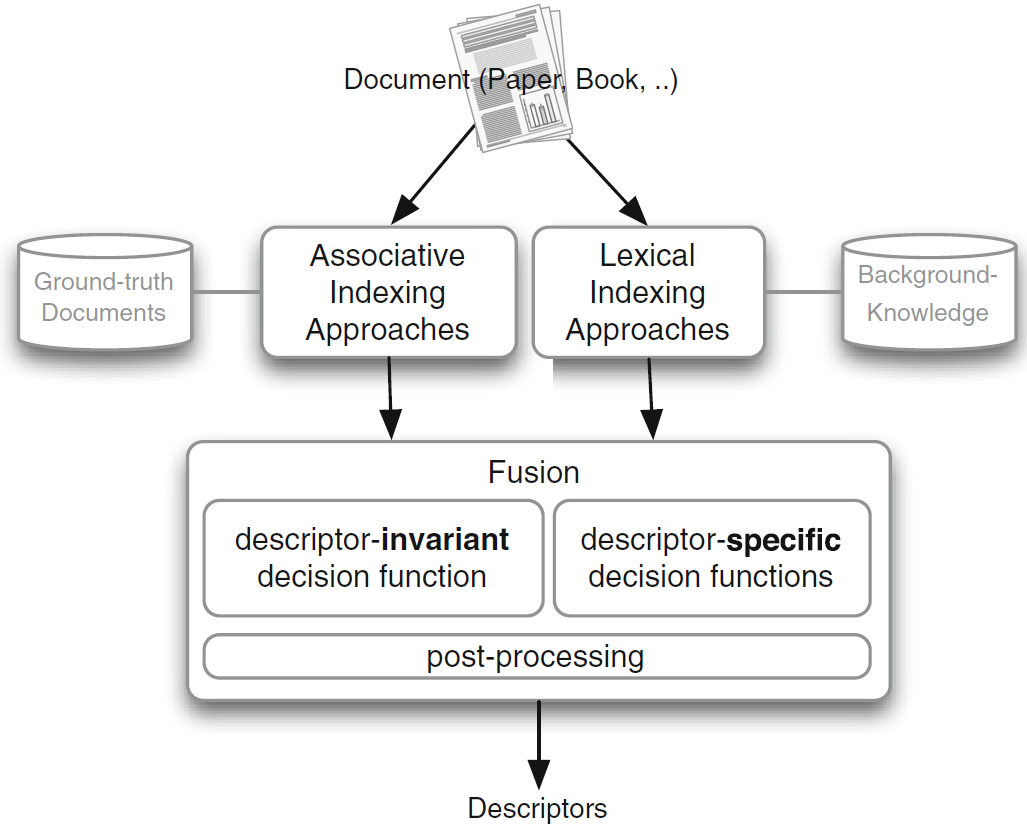
\includegraphics[width=.5\textwidth]{figures/related_work/fusion_architecture.PNG}
    \caption{Schema of a fusion architecture. From \cite{toepfer2020fusion}.}
    \label{fig:fusion_architecture}
\end{figure}

\textit{Fusion architectures} combine lexical and associative indexing systems. Their goal is to gather the advantages of both methods, which were shown to be complementary in the previous section, in one system. Figure \ref{fig:fusion_architecture} shows a schema of the architecture. The decision function, which can be either invariant or specific regarding the subjects, merges the results of the indexing systems into a single set of subjects, which is then assigned to the document after some optional post-processing. The descriptor-invariant decision function may be used for all descriptors, also unseen ones. The descriptor-specific decision function uses the background knowledge and the ground-truth documents to decide on the output.



\subsubsection{Comparison of classifications}

The usage of a \acrshort{kos} and the requirement of training data are the two distinguishing factors of the classifications. These are summarized in table \ref{tab:subject_indexing_classifications}. We will now look at them as a whole and establish relationships between them when possible.

\begin{table}
\centering
\begin{tabular}{|c|c|c|c|c|}
\hline
\thead{Author} & \thead{Group} & \thead{KOS} & \thead{Tr. data} & \thead{Method} \\
\hline\hline
\multirow{3}{*}{Golub} & Text categorization & Yes & Yes & ML algorithm \\ \cline{2-5}
& Document clustering & No & No & ML algorithm \\ \cline{2-5}
& Document classification & Yes & No & String matching \\ \cline{2-5}
\hline
\multirow{3}{*}{Medelyan} & Keyphrase extraction & No & No & String matching \\ \cline{2-5}
& Term assignment & Yes & Yes & Any \\ \cline{2-5}
& Keyphrase indexing & Yes & Yes & ML algorithm \\ \cline{2-5}
\hline
\multirow{3}{*}{Töpfer} & Associative methods & Yes & Yes & ML algorithm \\ \cline{2-5}
& Lexical methods & Yes & Yes & Both \\ \cline{2-5}
& Fusion architecture & Yes & Yes & Both \\ \cline{2-5}
\hline
\end{tabular}
\caption{Summary of the SI classifications.}
\label{tab:subject_indexing_classifications}
\end{table}

Golub's \textit{document clustering} and Medelyan's \textit{keyphrase extraction} are the only categories that require neither a \acrshort{kos} nor assigned documents as training data. They differ mainly in their objective: document clustering focuses on the subjects that relate documents, whereas keyphrase extraction looks at each document individually, looking for its most significant subjects.

Töpfer mentions Medelyan's models (KEA++ \cite{medelyan2008domain} and Maui \cite{medelyan2009human}) as examples of \textit{lexical methods}. Given that, according to Medelyan's classification, they belong to the \textit{keyphrase indexing} category, we can establish a relationship among these two categories. Furthermore, \textit{keyphrase indexing} arises from combining the other two categories of Medelyan's classification (\textit{term assignment} and \textit{keyphrase extraction}). Therefore, all three categories from Medelyan can be placed under Töpfer's lexical methods. Golub's \textit{text categorization} also requires training data and a \acrshort{kos}, and uses an \acrshort{ml} algorithm as well.

Finally, Medelyan mentions that \textit{term assignment} methods only require training data if an \acrshort{ml} algorithm is going to be used. If string matching is used, no training data is required. In this case, \textit{term assignment} would be equivalent to Golub's \textit{document classification} category, where the \acrshort{kos} is expected to be large enough for its entries to appear verbatim in the documents.

Considering all these similarities, we can identify three main types of \acrshort{si} methods. Those that require neither training data nor a \acrshort{kos}, those that only require a \acrshort{kos} and those that require both a \acrshort{kos} and training data.
\subsection{Challenges of Subject Indexing} \label{subject_indexing_challenges}

Here we present the common challenges faced by subject indexing approaches. They comprise the heterogeneity of the data, which increases the complexity of the task, as well as its size, which limits the implementation of machine learning approaches. The style of the texts, e.g. if they are scientific also impacts the performance of the approaches. Finally, we talk about the role of some characteristics of the subjects, such as how frequently they are assigned to documents, or their importance over time.

\subsubsection{Regarding the documents}

One important challenge is data heterogeneity \cite{kasprzik2020putting}. Because of the lack of strict standards, different users may introduce data into the repositories in different ways, which increases the complexity of performing \acrshort{si}. These issues have to be addressed through data cleaning and by developing models that are robust to noise.

The size of the dataset is often an obstacle for many methods. \cite{zhang2015character} believes that deep learning approaches only make sense when the training data exceeds 650 thousand examples. This estimate is confirmed by a subject indexing experiment \cite{mai2018using}, where the dataset that was well below the threshold was outperformed by the models trained on larger datasets.

Finally, the style of text, as well as its vocabulary and how technical it is, also play an important role. For instance, the developers of Annif \cite{suominen2019annif} state that its framework performs worse on technical fields where technical terms are frequent. They believe this is because of how precise such texts and terms are, in contrast with the broader meaning of concepts in humanities.

\subsubsection{Regarding the subjects}

The used subjects in the indexing task may also pose some difficulties for the indexing task. The first one is the different frequencies with which subjects are assigned to documents, where some subjects occur more often than others. This phenomenon can be explained with \textit{Zipf's law}: when ranked by frequency, the frequency of each subject is half of its predecessor \cite{toepfer2020fusion}.

This imbalance makes it difficult for models to learn when to assign subjects that rarely occur in the documents. Subjects that rarely occur are better assigned by unsupervised algorithms, whereas frequent subjects can be assigned with \acrlong{mlc} algorithms, as there are enough positive training example for the classifier to learn \cite{erbs2013bringing}. Another way of addressing this imbalance is to train independent binary classifiers for each subject, which provide more flexibility \cite{banerjee2019hierarchical}. However, this approach is only feasible when the number of subjects doesn't exceed a few hundreds because of its computational cost.

Another aspect of subjects that should be considered is how their assignment frequency changes over time \cite{toepfer2020fusion}. New subjects appear all the time, whereas others are slowly forgotten. For example, an institutional repository may have a lot of documents handling \textit{unsupervised learning} one year, but the research focus may shift towards \textit{supervised learning} the following year.

These changes in frequency affect the distribution of the subjects over time, which is used by statistical methods. Thus, a model that works well during development may fail to correctly assign subjects to new documents in the future if it does not adapt to the changes in the subject distribution. They can be addressed by combining statistical and matching approaches, as each covers the weaknesses of the other \cite{toepfer2020fusion}.

\subsubsection{Regarding the training data}

Supervised methods require examples of subject assignments from which to learn how subjects are mapped to documents. There are a couple of challenges that these training sets may pose.

The first problem may arise from the number of subjects. If it is too large, the required number of annotated documents significantly increases, as there are fewer documents representing each subject. This issue may also arise if the subjects form a complex hierarchy, where the subjects of the bottom levels are very specific and barely have any assignments. This issue is related to the different frequencies of subjects, which was stated above.

Another problem that often arises when using training data is the frequent contradictions that are contained in the documents. There is a lack of standard data collections, and using different annotations for a set of documents when training an \acrshort{ml} algorithm has been shown to lead to very different results \cite{yang1999evaluation}. According to a study involving 26 participants and 3 texts, the interpretations differed on about 40 \% \cite{morris2010individual}. Another example is given by \cite{medelyan2008domain}, which shows an agreement between indexers of 39 \%.

\subsection{Examples of unsupervised Subject Indexing} \label{subject_indexing_examples}

In this section, we will look at previous work that addresses \acrshort{si} with unsupervised approaches. The first one uses string matching to map subjects to documents, relying on the quality of the subjects to be thorough enough that multiple subjects can be found in any text. The second approach is the application of \acrlong{lda}, a probabilistic approach to topic modelling.

\subsubsection{String matching}

String matching methods rely on the quality and thoroughness of the \acrfull{kos} they use \cite{golub2019automatic}. A \acrshort{kos} is a special set of subjects where the subjects are structured, either in a hierarchy or through other kinds of relationships. The \acrlong{ddc} is an example of a  qualitative \acrshort{kos}. When the \acrshort{kos} covers all the relevant keywords that indicate that a document handles a certain topic, string matching methods may suffice to map subjects to documents. They are easier to implement and interpret, as well as cheaper to compute than more complex mapping functions, such as those optimized by machine learning algorithms.

An early application of this approach is the Wordsmith project \cite{godby2001wordsmith}. Its objective was to extract noun phrases from documents, which were then compared with the \acrfull{ddc} \acrshort{kos}. The authors thought that removing all other words during pre-processing would improve the accuracy of the indexing. Unfortunately, no significant difference in performance was observed.

Another project assigned \acrshort{ddc} terms to documents in unrelated libraries to facilitate cross-search \cite{khoo2015augmenting}. They achieved the best indexing results when using the title, the description and the keywords to represent each document. Their simple string matching approach took advantage of \acrshort{ddc} hierarchies for disambiguation to achieve competitive results, even when compared with \acrshort{ml} approaches that require annotated documents.
\subsubsection{Latent Dirichlet Allocation} \label{subject_indexing_lda}

Another unsupervised method that can be applied to subject indexing is \acrfull{lda} \cite{blei2003latent}. \acrshort{lda} is a probabilistic model where each document is given assignment probabilities for each of the subjects, describing it as a mixture of subjects. For example, a thesis about detecting tumors in medical images may be described as 70 \% \textit{machine learning} and 30 \% \textit{medicine}.

\acrshort{lda} finds the relationships between subjects and documents by computing the probability of each word belonging to each subject, while considering the words of the documents. Documents are represented as a mixture of topics, which in turn are represented as a mixture of words. The task of \acrshort{lda} is thus to split the individual words into groups semantically, i.e. where the words of each group have similar meanings. The output of \acrshort{lda} are then the composition of each subject as a mixture of words, and the assignment of those compositions, which are the subjects, to the documents.

The challenge when using \acrshort{lda} in subject indexing scenarios where a set of subject exists is that \acrshort{lda} does use any given subjects, but rather finds the subjects itself, as explained above. \cite{heryawan2021medical} addresses this issue by vectorizing the keywords of each subject output by \acrshort{lda}, as well as the subjects. The keywords and the subjects are then mapped in vector space with the cosine distance, which measures how similar the directions of the vectors are.

Their existing set of subjects was the set of medical subject headings (MeSH), which they assigned to a set of medical documents, represented either by their abstract or their full text. Their evaluation shows that the subjects output by \acrshort{lda} have an average cosine similarity of 74 \% to the MeSH subjects.



\subsection{Microsoft Academic Graph} \label{subject_indexing_mag}

The \acrfull{mag} is a knowledge base whose aim is to semantically relate scientific publications to one another \cite{shen2018web}. Its nodes can be of one of six types: publication, author, institution, journal, conference and concept. Having a high-quality concept model is detrimental and has been the main focus of Microsoft Research. The research group has developed throughout the past five years a concept hierarchy model which is used to semantically categorize scientific publications. Their pipeline comprises three steps. First, concepts are discovered; these concepts are then assigned to documents when semantically appropriate; finally, the relationships between the documents are used to build a concept hierarchy. We will now look at each of these steps more in detail.

\begin{table}
\begin{center}
    \begin{tabular}{| p{1.6cm} | p{2.9cm} | p{2.7cm} | p{2.3cm} |} 
    \hline
     & \thead{Concept \\ discovery} & \thead{Concept \\ tagging} & \thead{Hierarchy \\ building} \\ [0.5ex] 
    \hline\hline
    \thead{Problem} & \makecell{knowledge base \\ type prediction} & \makecell{multi-label text \\ classification} & \makecell{topic hierarchy \\ construction} \\ 
    \hline
    \thead{Solution} & \makecell{graph link analysis \\ on Wikipedia} & \makecell{word embeddings \\ + \\ graph structure} & \makecell{extended \\ subsumption} \\
    \hline
    \thead{Test \\ accuracy} & \makecell{94.75 \%} & \makecell{81.20 \%} & \makecell{78.00 \%} \\
    \hline
    \end{tabular}
    \caption{Summary of each phase of the \acrshort{mag} development.}
    \label{tab:mag}
\end{center}
\end{table}

Before introducing each of these steps, we explain the word embedding model they use, called skip-gram \cite{mikolov2013distributed}, which is the key component of their procedure. The word embeddings are trained by comparing them with the embeddings of the word that surround it in the text. Thus, embeddings are trained locally, focusing on the context of each word, rather than globally, where statistics and other metrics that consider the data as a whole are introduced.

After outlining \acrshort{mag}'s three steps, we introduce the two ways in which its data can be accessed. The \acrfull{makg} \cite{faerber2019microsoft} offers the data in RDF files, which are suitable for analysis tasks and efficient exploration. The second option is an expressive \acrshort{api}, provided by OpenAlex, which offers granular access to the documents and subjects. It also includes all the subject assignments, whereas the \acrshort{makg} only assigns fields. Therefore, we will use OpenAlex in this thesis.

\subsubsection{Skip-gram} \label{mag_skipgram}

The key component of Microsoft's approach is Skip-gram \cite{mikolov2013distributed}, a model for representing words as vectors, called embeddings. The embeddings are improved by training the model. The model receives the center word, and it should predict the context words. How many context words the model should be able to predict depends on the window size. We have implemented skip-gram in PyTorch\footnote{\url{https://github.com/carlosfranzreb/skipgram}}. Details about the training procedure and examples of embeddings can be found in section \ref{implementation_skipgram}.

Skip-gram arises as a counterpart to the \acrfull{cbow} model. This model is trained by giving it the words surrounding a certain word as input, called context words. It then has to predict the center word, i.e. the word that is surrounded by the context words in the data. Skip-gram was an improvement in both training time and semantic quality of the representation, according to the experiments of the authors \cite{mikolov2013efficient}.

The initial model was improved by adding two features. The first is subsampling of frequent words. The representation of words that appear often doesn't change much after a while, as the model has already tuned them. On the other hand, words that seldom appear on the data need more iterations for their representations to achieve a comparable accuracy. Therefore, frequent words are subsampled according to the formula below, which aggressively discards words whose frequency exceeds the threshold $t$. This increases accuracy, as the model doesn't overfit frequent words.

$$ Discard(word) = 1 - \sqrt{\frac{t}{freq(word)}} $$

The second improvement to the model was the introduction of negative sampling. It alleviates the computational cost of the problem, which, without negative sampling, requires computing the softmax of all data points. With negative sampling, we only consider $k$ words other than the input words, called negative samples. We assume that their vector representations should be considerably different from the representation of our input word. Thus, the model should output zero when fed the input word and one of the negative samples.
\subsubsection{Concept discovery} \label{mag_concept_discovery}

Given the vast amount of publications that appear every year (a number that doubles every dozen years \cite{dong2017century}), manually curating concepts is not a possibility anymore. A large amount of concepts is needed to properly characterize every document. Temporal dynamics (i.e. how research focus shifts over time) should also be monitored. This requires regular updates of the concept model, which again hinders the manual approach to solving the task.

Microsoft Research has adopted a hybrid approach for discovering concepts. They have manually defined the first two levels of the concept model (i.e. the two broadest levels) as well as 2000 other high-quality concepts, and solved the \textit{knowledge base type prediction} problem to assist them in discovering more specific concepts from the Wikipedia knowledge base. Their approach iterates between \textit{graph link analysis} for discovering potential concepts and \textit{entity type based filtering and enrichment}, which selects the most appropriate concepts out of the candidates retrieved in the previous step. The iteration is executed a few times, without any particular stopping criterion.

Graph link analysis explores concept candidates by assuming that the nearest neighbors of a concept are also concepts. Similarity between Wikipedia entities is defined based on the amount of hyperlinks to other entities that they share \cite{witten2008effective}. In the second step of the loop, the candidate concepts are filtered based on their type. Entities that belong to types which are irrelevant for the concept model, such as \textit{person}, are removed. Then, all other Wikipedia entities of the remaining types are added to the list of candidates. Which types are valid is determined using an undisclosed knowledge base.
\subsubsection{Concept tagging} \label{mag_concept_tagging}

Tagging concepts to publications is performed by solving a multi-label classification problem. Heuristics are applied to reduce the number of candidate pairs between concepts and publications, as evaluating every possible pair is unfeasible. All concepts of the first two levels as well as the concepts present in the publication's \acrfull{ert} are included in the classification task. The \acrshort{ert} is an extension of the text that describes an entity, termed \acrfull{srt}, to include textual information from its neighboring nodes in the \acrshort{mag}. Four representations of each \acrshort{ert} are concatenated and used as its vector representation: bag-of-words, bag-of-entities, embedding-of-words and embedding-of-entities. Words are also embedded as vectors using a skip-gram model \cite{mikolov2013distributed} that was pre-trained on an academic corpus.

To assign an \acrshort{ert} to each concept, the authors first manually assigned venues to concepts. The \acrshort{ert} of each concept is then the aggregation of the \acrshort{ert}s of the venues it was assigned. The mapping of venues to concepts is not available online. Once all publications and concepts are embedded (both as \acrshort{ert}s), a confidence score for each pair of concept and \acrshort{ert} is computed as the cosine similarity between their vector representations. The authors computed confidence scores for 50 billion pairs and kept one billion of them.
\subsubsection{Hierarchy building} \label{mag_hierarchy_building}

Once the publications have been tagged with the concepts, they can be used to extract a hierarchy for the concepts. The authors use \textit{subsumption} for this purpose, which assumes that concept $x$ subsumes concept $y$ if $y$ only occurs in a subset of the publications where $x$ occurs \cite{sanderson1999deriving}. The condition can be relaxed; $y$ is considered a child of $x$ in the hierarchy if both terms co-occur in a certain proportion of publications, i.e. 75 \%. The authors extend this method by including the confidence scores for the pairs of concepts and publications computed in the previous phase.

The resulting subsumption model was used to construct a six-level hierarchy of concepts. The relationships between the concepts of the first two levels were adjusted manually. All other relationships were left as they were output by the model. A limitation of this model, which translates to a worse accuracy (see table \ref{tab:mag}), is that relationships are not always transitive. For example, Fernando Alonso is a Formula 1 driver, which is a profession, but the relationship between ``Fernando Alonso'' and ``profession'' is unclear. The authors stated that they plan on addressing this issue by including information about the types of the entities.
\subsubsection{Updates since the paper's publication} \label{mag_updates}

Last year, the research group posted a blog post\footnote{\url{https://www.microsoft.com/en-us/research/project/academic/articles/expanding-concept-understanding-in-microsoft-academic-graph/}} highlighting some changes to the methods described above. There were two major updates to the phase of discovering concepts, which we discuss in this section. These two updates increased the number of concepts from 227 thousand to over 700 thousand. The second update is also performed regularly to discover new topics.

The first update consisted of adding concepts from the biomedical domain using the  Unified Medical Language System (UMLS) vocabulary. Biomedical concepts from the (UMLS) that were relevant to the corpus (regarding term frequency) were added to the concept model. This procedure was performed only once. The second update is the paradigm shift for topic discovery. Instead of retrieving concepts from Wikipedia, the new approach directly extracts concepts from the academic literature. It consists of two steps.

\begin{enumerate}
    \item Identify words or phrases in the text of the publications that are concepts (without stating which specifically). This problem is called \textit{sequence labeling}. The authors' approach consists of doing lexical matching on a sample of \acrshort{mag} publications using the synonyms of existing concepts to generate a training set. This set is then fed to a transformer as a context encoder and a conditional random field as a tag decoder to train a binary classifier on each word.
    \item Differentiate between existing, new and low-quality concepts by evaluating the relevance of the URLs returned by the Bing Web Search \acrshort{api} when looking for the concept. Equivalent concepts are grouped together.
\end{enumerate}

\subsubsection{Accessing the data} \label{mag_access_data}

Microsoft provides \acrshort{api} access\footnote{\url{https://docs.microsoft.com/en-us/academic-services/project-academic-knowledge/reference-evaluate-method}} to their corpus, including already tokenized abstracts and the subjects of each document. A subscription is required to access the \acrshort{api} endpoint and the rate limit is set to 10,000 transactions per month and 1 per second. Unfortunately, the \acrshort{mag} service was shut down at the end of 2021. We therefore discuss two other options, that also offer \acrshort{mag} data, in the following sections. We then close this chapter by arguing our choice between them.

\paragraph{MAKG} \mbox{}

Michael Färber has processed the data from the papers and offers dump files in \acrfull{rdf} format \cite{faerber2019microsoft} and also provides an SPARQL endpoint\footnote{\url{https://makg.org/sparql}}. Each file includes different information, such as metadata about the subjects, the authors or the papers. The abstracts have also been reconstructed into free text, as Microsoft only provides them as lists of tokens.

Färber's dumps comprise over 238 million publications and 740,460 subjects\footnote{These numbers refer to the dump of 29.05.2020}. How the subjects are distributed among the fields (i.e. the subjects of the first level) is displayed in figure \ref{fig:subjects_per_field_per_level}. This plot only considers the subjects that are part of the hierarchy. There are 196,631 subjects (27 \%) that do not belong to any of the fields.

341,959 subjects of the hierarchy (46 \%) belong to the fields of biology and medicine. Environmental science is the least represented field, with only 126 subjects, followed by history, which comprises 1,510 subjects. Regarding the levels, there are 19 subjects in the first level (called fields from now on) and 292 in the second. The latter ones include over 100,000 subjects per level, incrementally increasing and peaking at 165,321 subjects in the sixth level.

\begin{figure}
    \centering
    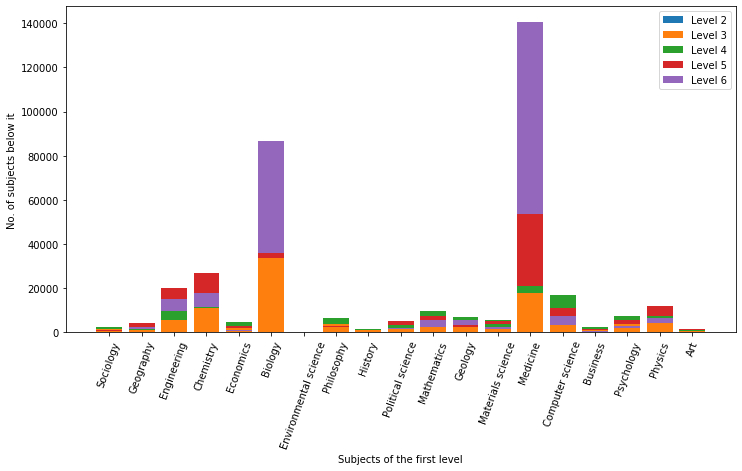
\includegraphics[width=\textwidth]{figures/related_work/makg/subjects_per_field_per_level.png}
    \caption{Subjects present in the MAKG.}
    \label{fig:subjects_per_field_per_level}
\end{figure}

\begin{figure}
    \centering
    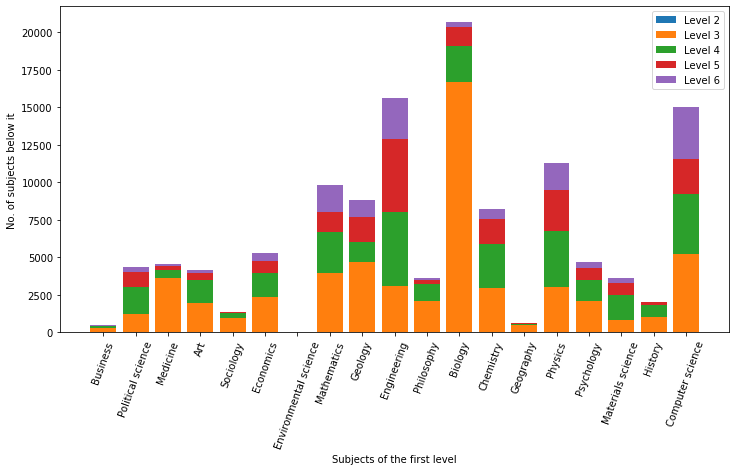
\includegraphics[width=\textwidth]{figures/related_work/makg/subjects_w_article.png}
    \caption{Subjects of the MAKG that have a Wikipedia link.}
    \label{fig:subjects_w_article}
\end{figure}

\begin{figure}
    \centering
    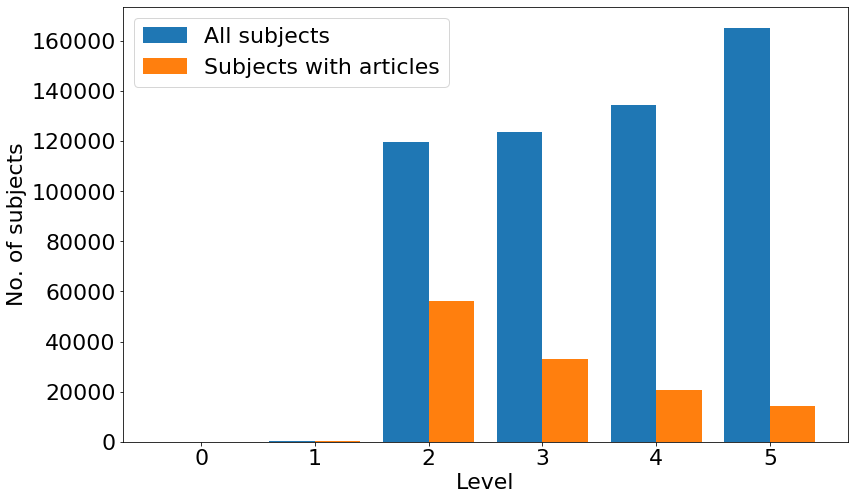
\includegraphics[width=.75\textwidth]{figures/related_work/makg/subject_distribution_comparison.png}
    \caption{Comparison of all subjects with the subset that have a Wikipedia link.}
    \label{fig:subject_distribution_comparison}
\end{figure}

124,385 subjects (17 \% of all subjects) have a Wikipedia link. These are shown in figure \ref{fig:subjects_w_article}. They are relevant for computing the vector representations of the subjects. If they are not present, we cannot do so, as we don't have a text associated to the subject we can use for the vectorization procedure. Biology is the field with the most links, followed by Computer Science and Engineering. Only 4,574 subjects of the 179,741 in the field of Medicine (2.5 \%) have a link, which is why this field is no longer the most populated field when considering Wikipedia links. The difference among all subjects and those with links is shown in figure \ref{fig:subject_distribution_comparison} on a per-level basis. When looking at all subjects, the number increases with the level. When looking at the subjects with links, the opposite occurs: the number of subject decreases with the level.

Regarding the subject assignments of the documents, Färbers files don't include all the subjects assigned to each document. When querying the SPARQL endpoint for all subjects that have been assigned to at least one paper, only 19 subjects are returned. They are very broad subjects, such as \textit{Geology} or \textit{Computer Science}. The assigned subjects in Färbers \acrshort{rdf} files also don't always coincide with the ones assigned by Microsoft. For example, in the \acrshort{rdf} files the paper \textit{Determination of vitamin D3 and 25-hydroxyvitamin D3 in foodstuffs by HPLC UV-DAD and LC–MS/MS} has the subject \textit{Environmental Science}, whereas in Microsoft Academic the topics assigned to the publication include \textit{Vitamin}, \textit{High-performance liquid chromatography} and eight others. These subjects can be retrieved through the \acrshort{api}.
\paragraph{OpenAlex} \mbox{}

OpenAlex\footnote{\url{https://openalex.org/about}} is the successor of the \acrshort{mag}. It offers the whole \acrshort{mag}, combined with several other sources, through a RESTful \acrshort{api}. It arose because the \acrshort{mag} was shut down by Microsoft at the end of 2021, which opened the door for other companies to fill the gap. OpenAlex is still on beta release, which they plan to emerge from in the upcoming months. However, it currently has all the data that \acrshort{mag} had, and more. It also imports data from sources like Crossref\footnote{\url{https://www.crossref.org/}}, ORCID\footnote{https://orcid.org/} and PubMed\footnote{https://pubmed.ncbi.nlm.nih.gov/}.

Among numerous interesting features, it allows searching for publications that are assigned a certain subject. When retrieved from the API, subjects includes the \acrshort{api} request to retrieve its corresponding publications, as well as the number of publications it is assigned to. We can use this number to assess the relevance of a subject. Subjects also include a list with all its ancestors, which we can use to navigate the hierarchy. The \acrshort{api} offers several filters when querying subjects, such as hierarchy level and ancestors.
\paragraph{Choice of data source} \mbox{}

The two options, \acrshort{makg} and OpenAlex, offer different services. \acrshort{makg} stores the \acrshort{mag} data as \acrshort{rdf} triples, which are suited for exploring the knowledge graph through its entities, integrating the \acrshort{mag} data with other sources and performing large scale data analysis \cite{faerber2019microsoft}. OpenAlex, on the other hand, offers a variety of filters to construct granular \acrshort{api} requests, which makes the data very accessible. However, it is not as scalable as the \acrshort{makg}, which can be navigated efficiently with SPARQL.

The main drawback of \acrshort{makg}, which renders it useless for our use case, is that it does not include the assignments of subjects to documents. It only includes the assignment of publications. We require these assignments to build a dataset of documents and their assigned subjects, which we then use to train a supervised classifier. OpenAlex does offer all the assignments that are present in \acrshort{mag}, and therefore is our choice as the data source for subjects and training data. Given that we only require basic filtering and don't want to perform any large scale analysis, we do not require the scalability that \acrshort{rdf} triples offer. The \acrshort{api} objects that OpenAlex outputs fulfill all our requirements.


